\documentclass[12pt]{article}
\usepackage{fullpage}
\usepackage{graphicx} % for include picture
% this package include subfigure
\usepackage{subcaption}
% very useful for citation
\usepackage[]{amsmath}
\usepackage{enumerate}

\usepackage{algpseudocode}
% algorithm pseudocode package http://en.wikibooks.org/wiki/LaTeX/Algorithms#Typesetting_using_the_algorithmic_package
% include python codes
\usepackage{listings}
\usepackage[T1]{fontenc}
\usepackage[scaled]{beramono}
% for latex tables
\usepackage{booktabs}
\usepackage[colorlinks = true,
  linkcolor = blue,
  urlcolor  = blue,
  citecolor = blue,
anchorcolor = blue]{hyperref}

%must be loaded at last
\usepackage{cleveref}

\title{The tile of the report}

\author{Author XXX}

\begin{document}
\maketitle
\date
\noindent

\section*{Example of enumeration and itemization}
\label{section 1}
\begin{enumerate}
  \item item 1.
    \begin{itemize}
      \item item 1.
      \item item 2.
    \end{itemize}
  \item item 2.
\end{enumerate}

% \begin{figure}[h]
%   \centering
%   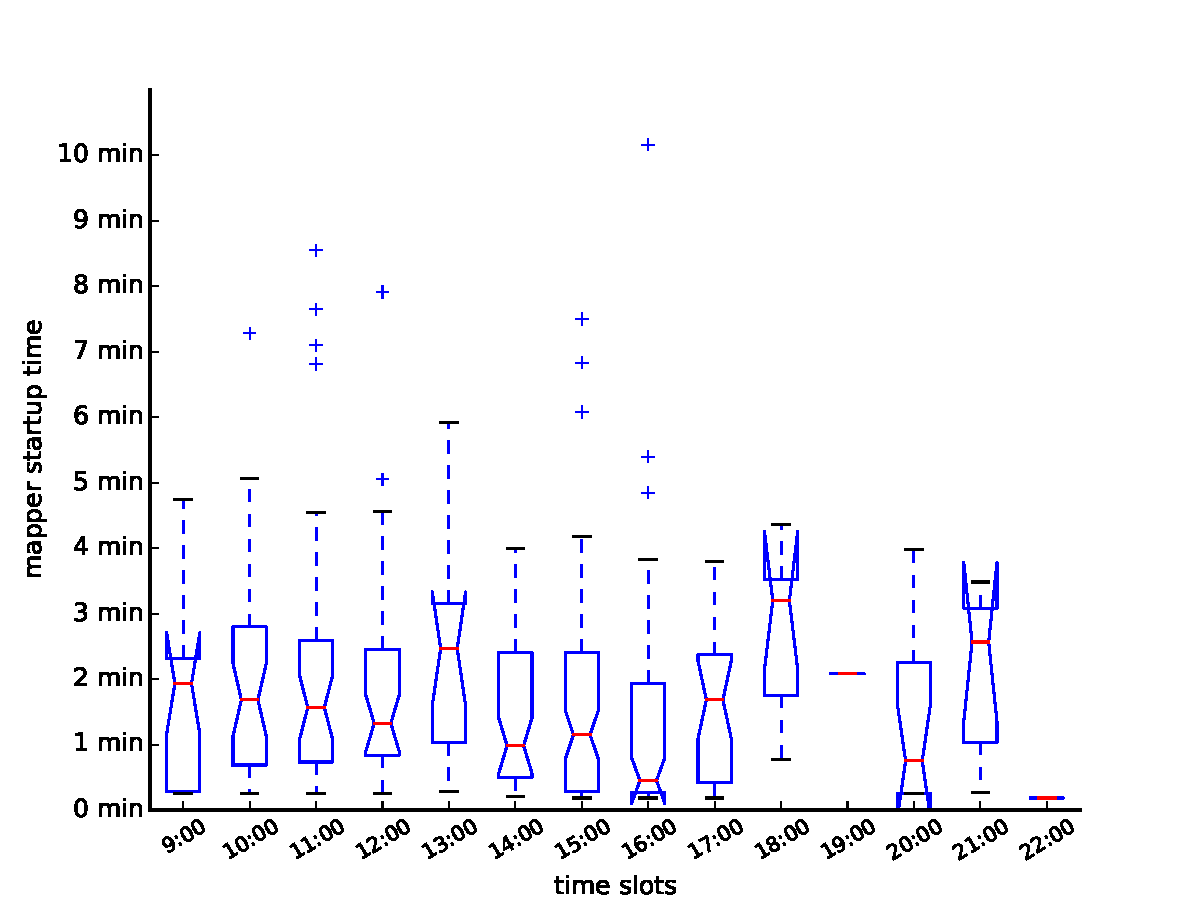
\includegraphics[width=.7\textwidth]{mapper_startup_time_distribution.pdf}
%     % \scriptsize
%   \caption{Mapper Startup time V.S. different time slots within a day}
%   \label{fig:mapper}
% \end{figure}

% \begin{figure}[h]
%   \centering
%   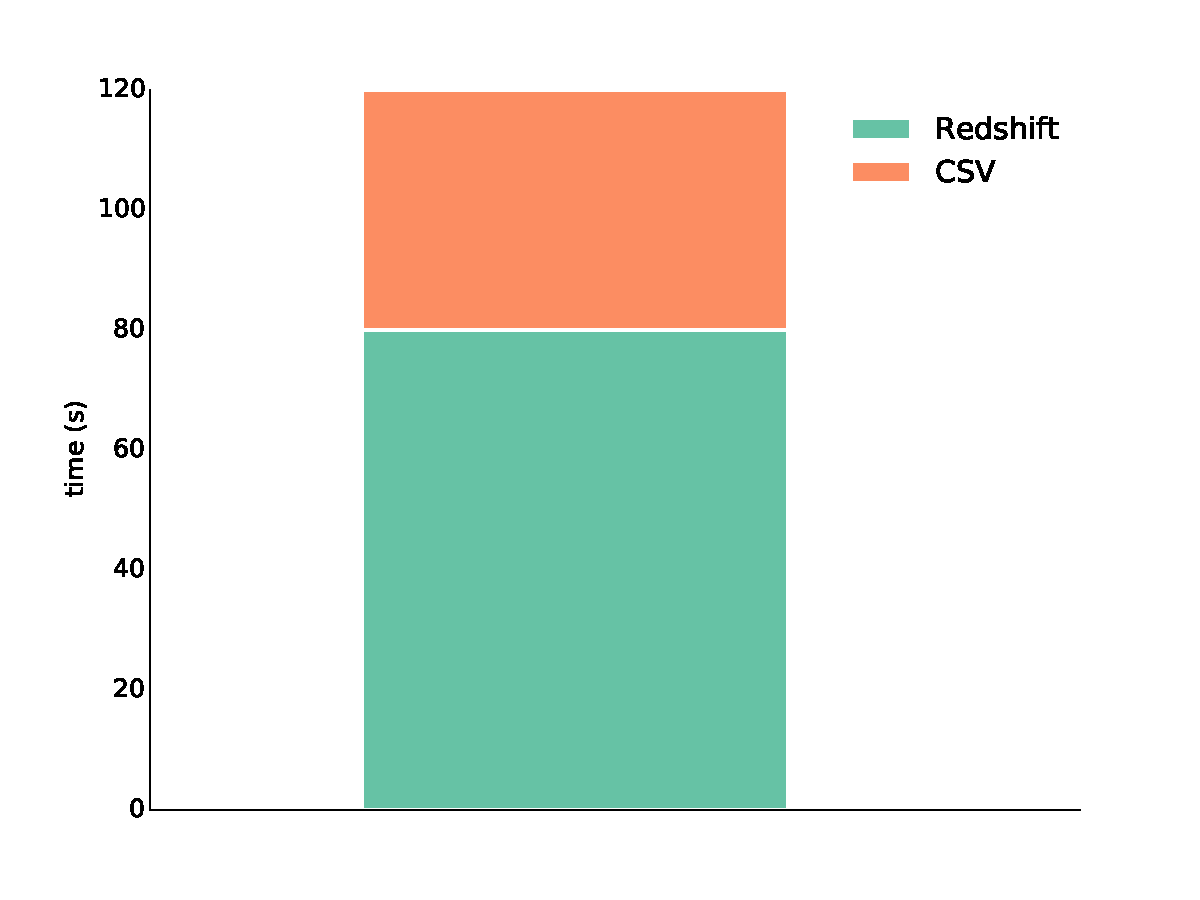
\includegraphics[width=\textwidth]{RedshiftCSV_bar.pdf}
%     % \scriptsize
%   \caption{Mapper Startup time breakdown}
%   \label{fig:breakdown}
% \end{figure}

\begin{figure}[tb]
  \centering
  \begin{subfigure}{.8\textwidth}
    \centering
    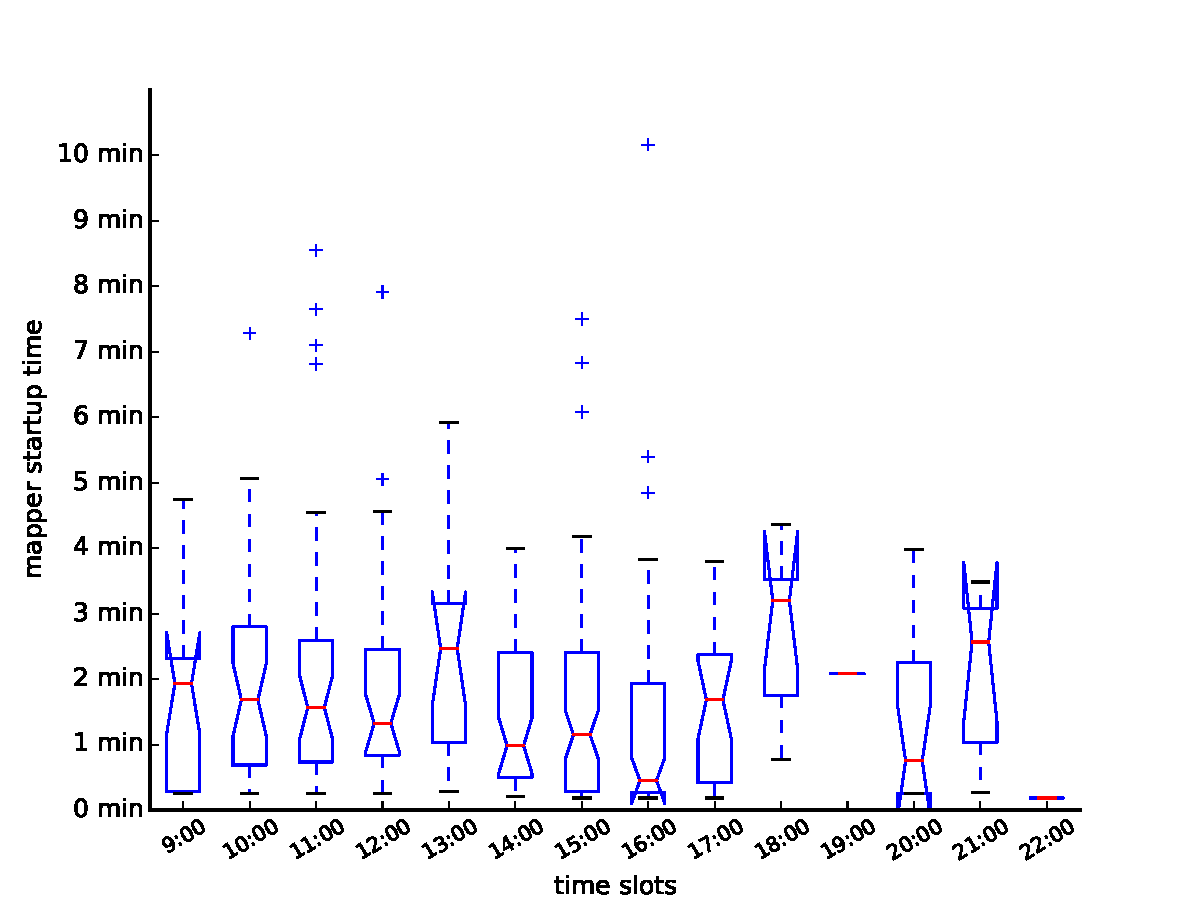
\includegraphics[width=\textwidth]{mapper_startup_time_distribution.pdf}
    \caption{Mapper Startup time distributions during different times of a day}
    \label{fig:mapper}
  \end{subfigure}
  \begin{subfigure}{.8\textwidth}
    \centering
    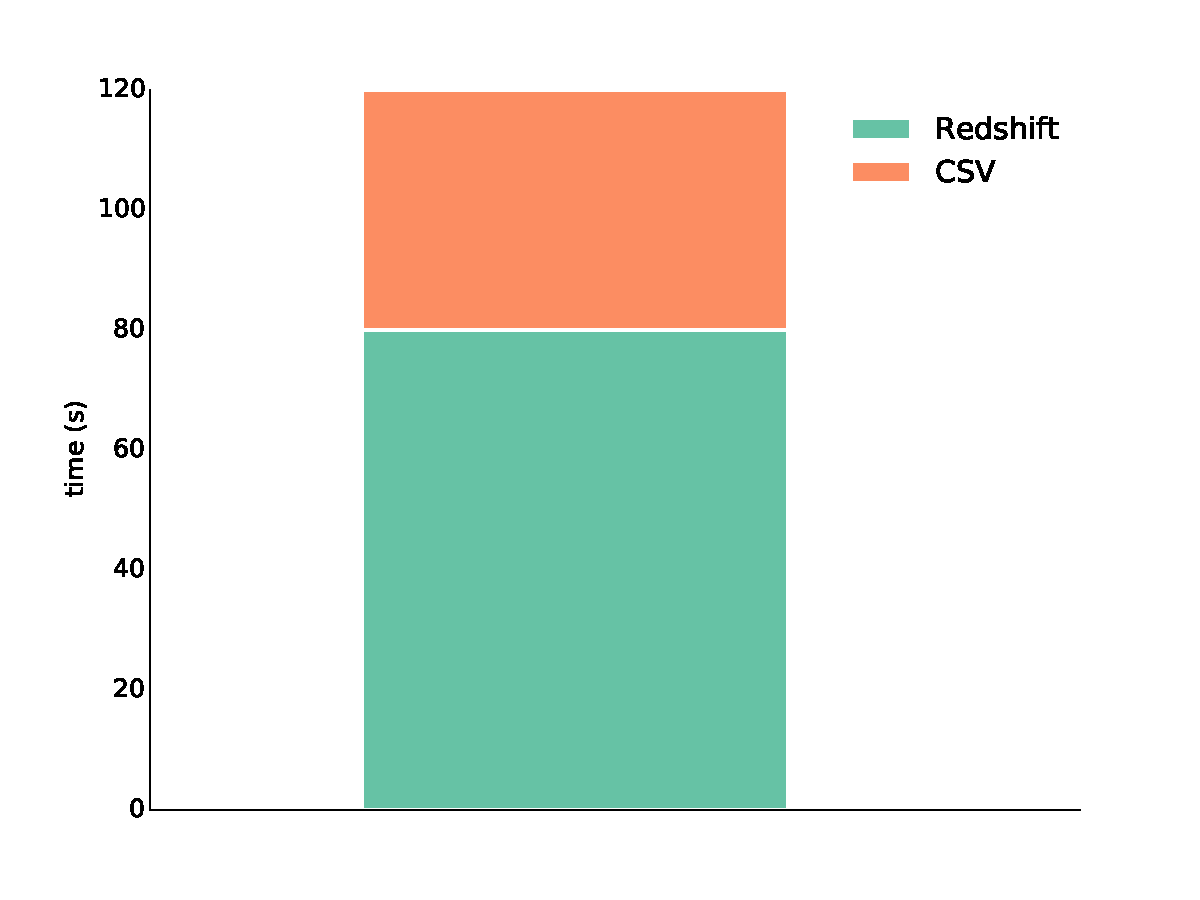
\includegraphics[width=\textwidth]{RedshiftCSV_bar.pdf}
    % \scriptsize
    \caption{Mapper Startup time breakdown}
    \label{fig:breakdown}
  \end{subfigure}
  \caption{}
\end{figure}




\section*{Referencing figure and tables}
\Cref{tab:time_probability} is a table showing \dots. \\

\begin{table}[h]
  \centering
  \begin{tabular}{cc}
    \toprule
    probability &  time cost (min) \\
    \midrule
    0.450 &          1 \\
    0.657 &          2 \\
    0.851 &          3 \\
    0.927 &          4 \\
    0.958 &          5 \\
    0.971 &          6 \\
    0.979 &          7 \\
    0.992 &          8 \\
    0.995 &          9 \\
    0.995 &         10 \\
    \bottomrule
  \end{tabular}
  \caption[Probabilities of mapper finishing startup before certain time
  period has elapsed]{Probabilities of mapper finishing startup before certain time
  period has elapsed}
  \label{tab:time_probability}
\end{table}

\Cref{fig:mapper} is showing how to referencing a figure. \\
\Cref{fig:breakdown} is showing a breakdown of \dots.

\section*{Footnotes}
The chance of mapper takes longer than 10 min to finish startup is <
0.005\% \footnote{This conclusion is drawn from the data on my virtual box,
which has 378 rows of data collected since August}.

\section*{URL links}
\href{url}{This is a URL link.}

\end{document}

%% Local Variables: 
%%% mode: latex
%%% TeX-master: t
%
